\subsection{Random walks and arithmetic brownian motion}
Imagine starting at the origin of a Cartesian plane and, every second, having the same probability of moving east, west, north, south (or even in a oblique direction). After a certain number of steps, the position you end up in is \textbf{completely unpredictable}. A \textbf{random} \textbf{walk} is a path constructed in this way, with a sequence of steps determined by probability. \\
\\
Key characteristics of a random walk:
\begin{itemize}
    \item \textbf{Unpredictable and independent increments}: Previous steps have no influence on future ones.
    \item \textbf{Variance that grows over time}: The number of possible final positions after $n$ steps increases as $n$ increases. (With a bit of reasoning, one can see that it grows proportionally to $\sqrt{n}$).
    \item \textbf{In the case of no drift}: on average, you end up at the starting point (each direction has equal probability).
\end{itemize}
We say that a random walk is driven (has a drift) when the directions have different probabilities.
%\begin{figure} [H]
%        \centering
%        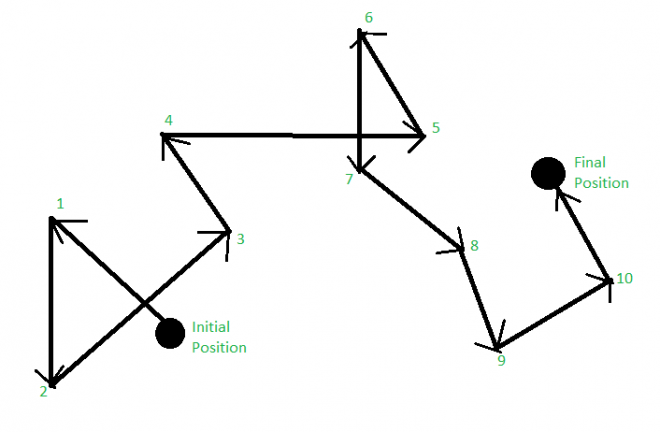
\includegraphics[width=0.5\linewidth]{img/random_walk_1.png}
%        \caption{Example of a 2D random walk}
%    \end{figure}
%\begin{figure} [H]
%    \centering
%    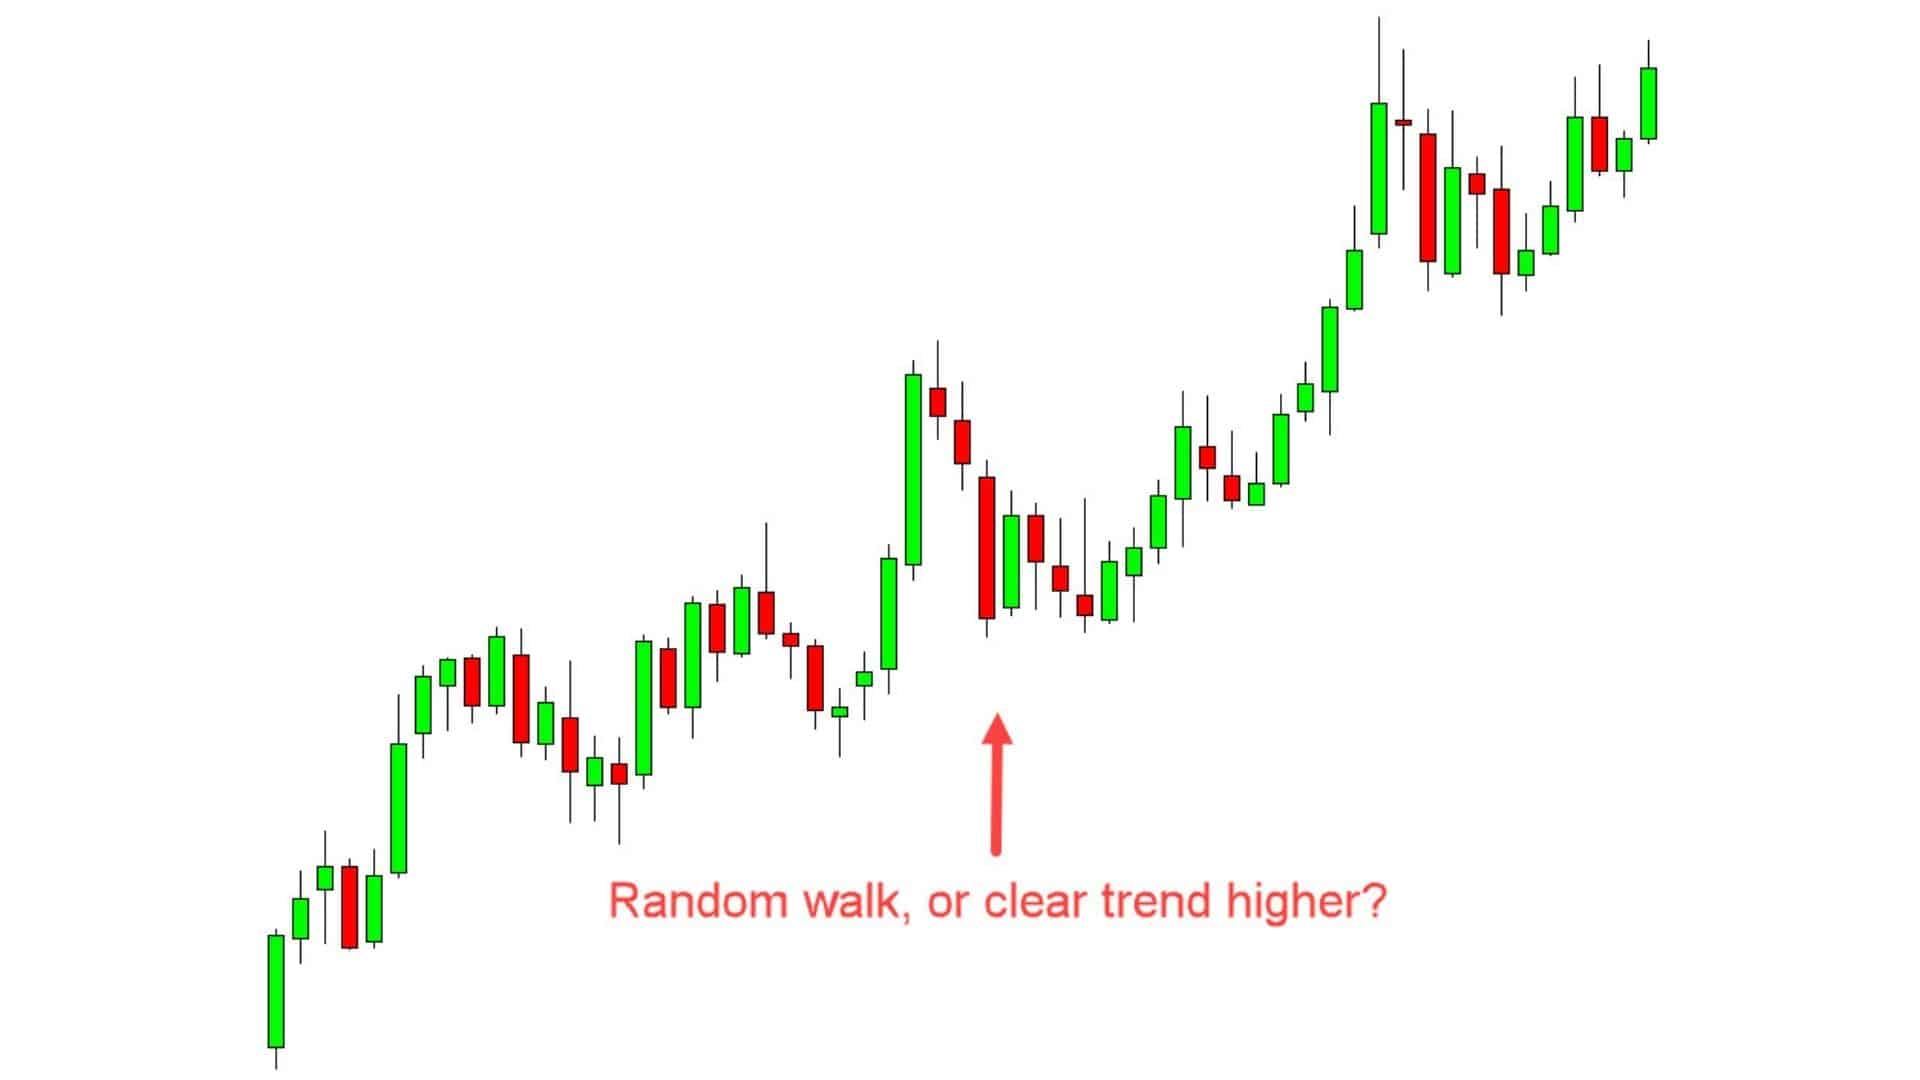
\includegraphics[width=0.75\linewidth]{img/random_walk_2.png}
%    \caption{Could one see the market as an example of a 1D random walk?}
%\end{figure}


\begin{figure}[H]
    \centering
    \begin{subfigure}{0.47\textwidth}
        \centering
        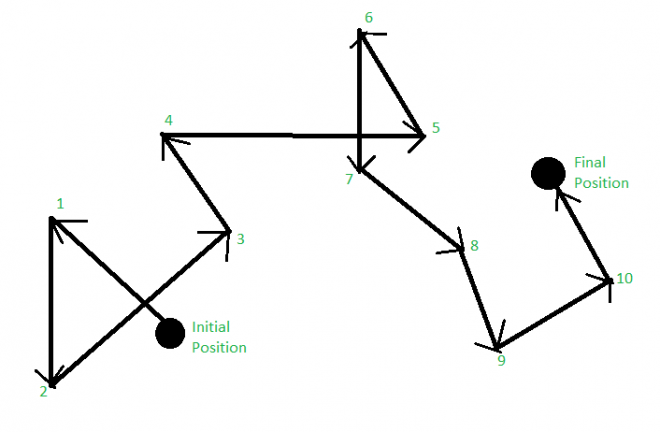
\includegraphics[width=\linewidth]{img/random_walk_1.png}
        \caption{Example of a 2D random walk.}
        \label{fig:sub1}
    \end{subfigure}
    \hfill
    \begin{subfigure}{0.47\textwidth}
        \centering
        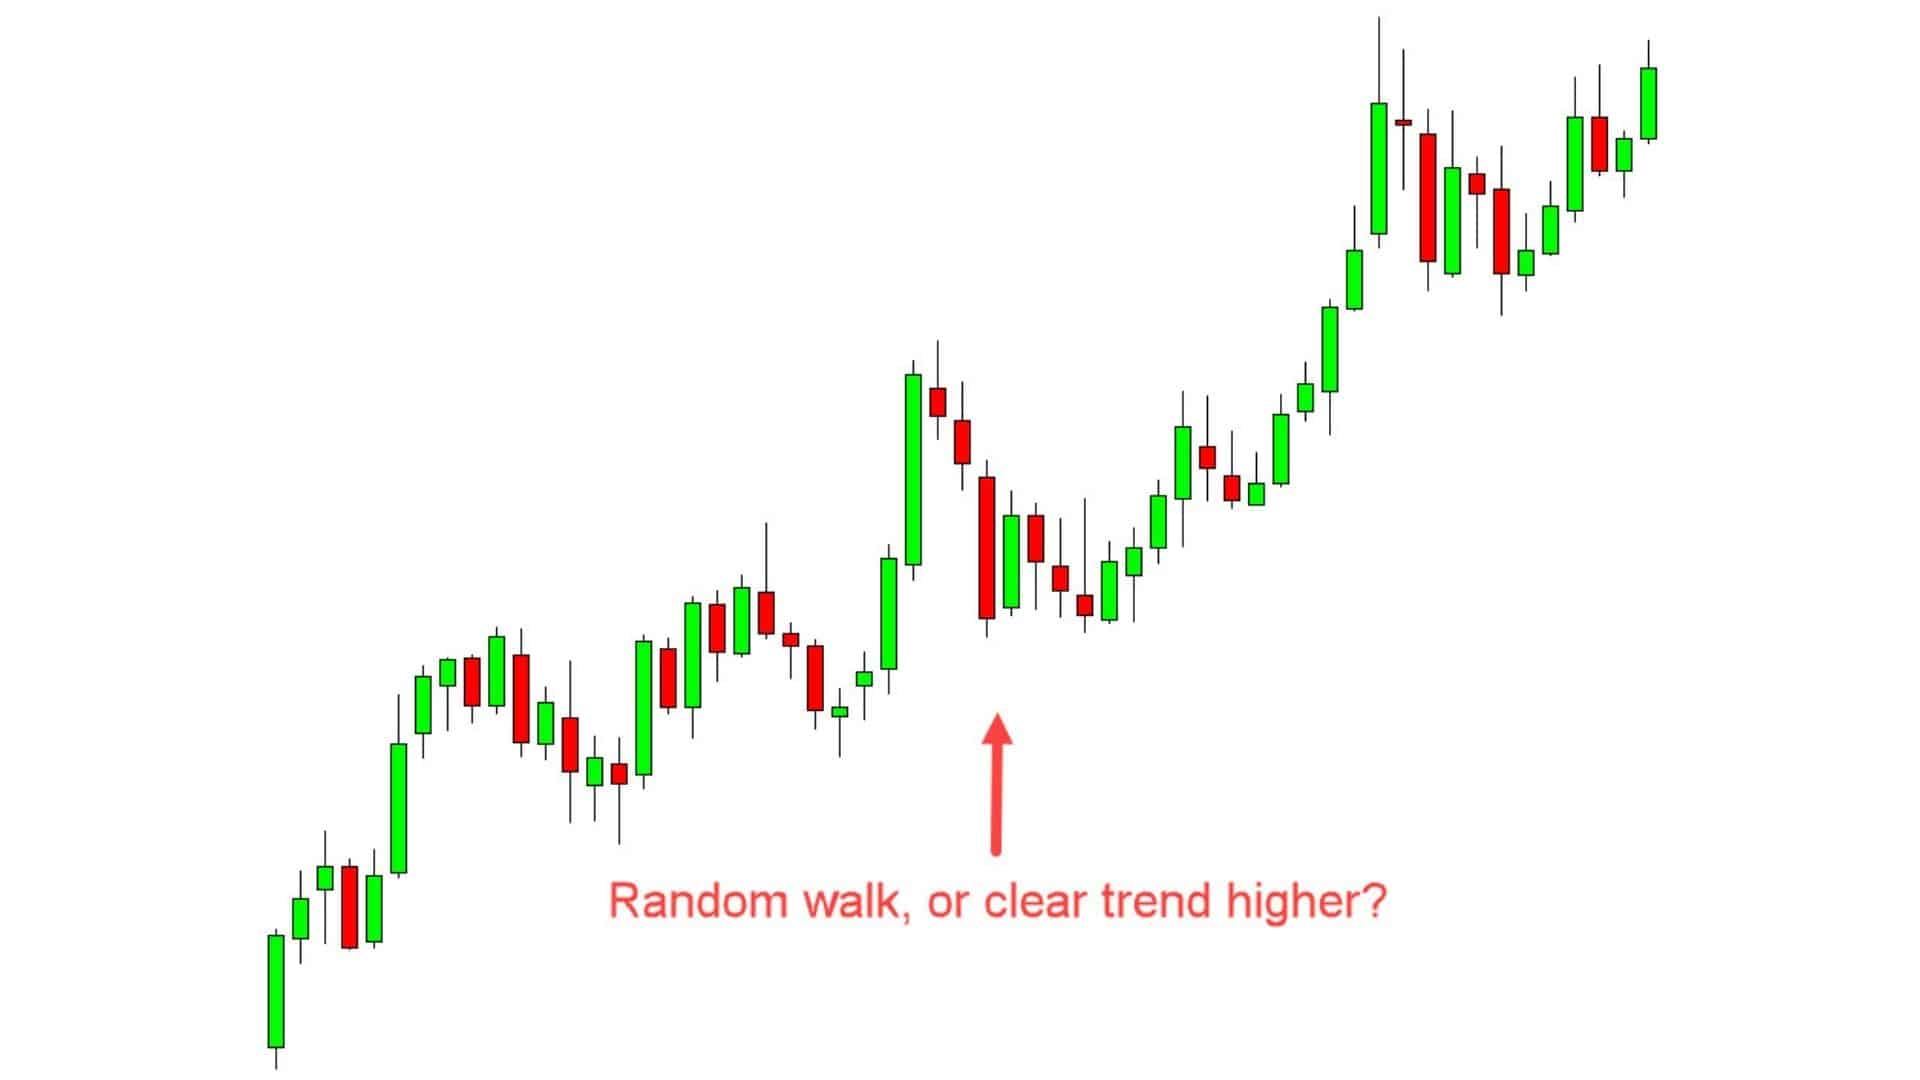
\includegraphics[width=\linewidth]{img/random_walk_2.png}
        \caption{Is the market a 1D random walk?}
        \label{fig:sub2}
    \end{subfigure}
    \caption{Examples of random walks.}
    \label{fig:due_immagini}
\end{figure}

\textbf{Arithmetic Brownian motion}: is the random motion of particles suspended in a liquid or gas medium. It consists of random fluctuations in a particle's position inside a fluid. In a fluid at thermal equilibrium there exists no preferential direction of flow (i.e. with no drift). \\
Basically the arithmetic brownian motion is a continuous-time process with Gaussian increments, essentially a continuous analogue of the random walk.\\

If you take a random walk and rescale it properly (step size $\Delta t \to 0)$ and consider jumps proportional to $\sqrt{\Delta t}$ then in the limit you obtain a Brownian motion.

\begin{figure} [H]
    \centering
    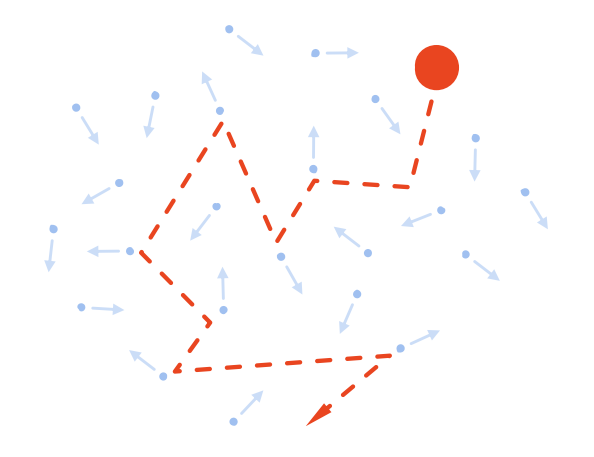
\includegraphics[width=0.5\linewidth]{img/brownian_motion.png}
    \caption{Illustration of the brownian motion of a sphere inside a fluid.}
\end{figure}

\subsection{Bachelier model}
In 1900, \textbf{Bachelier} proposed that stock prices follow a \textbf{random walk with no drift}, implying that their distribution is \textbf{normal} with a \textbf{variance proportional to time} (see Appendix \ref{app:A}).
\begin{figure} [H]
\centering
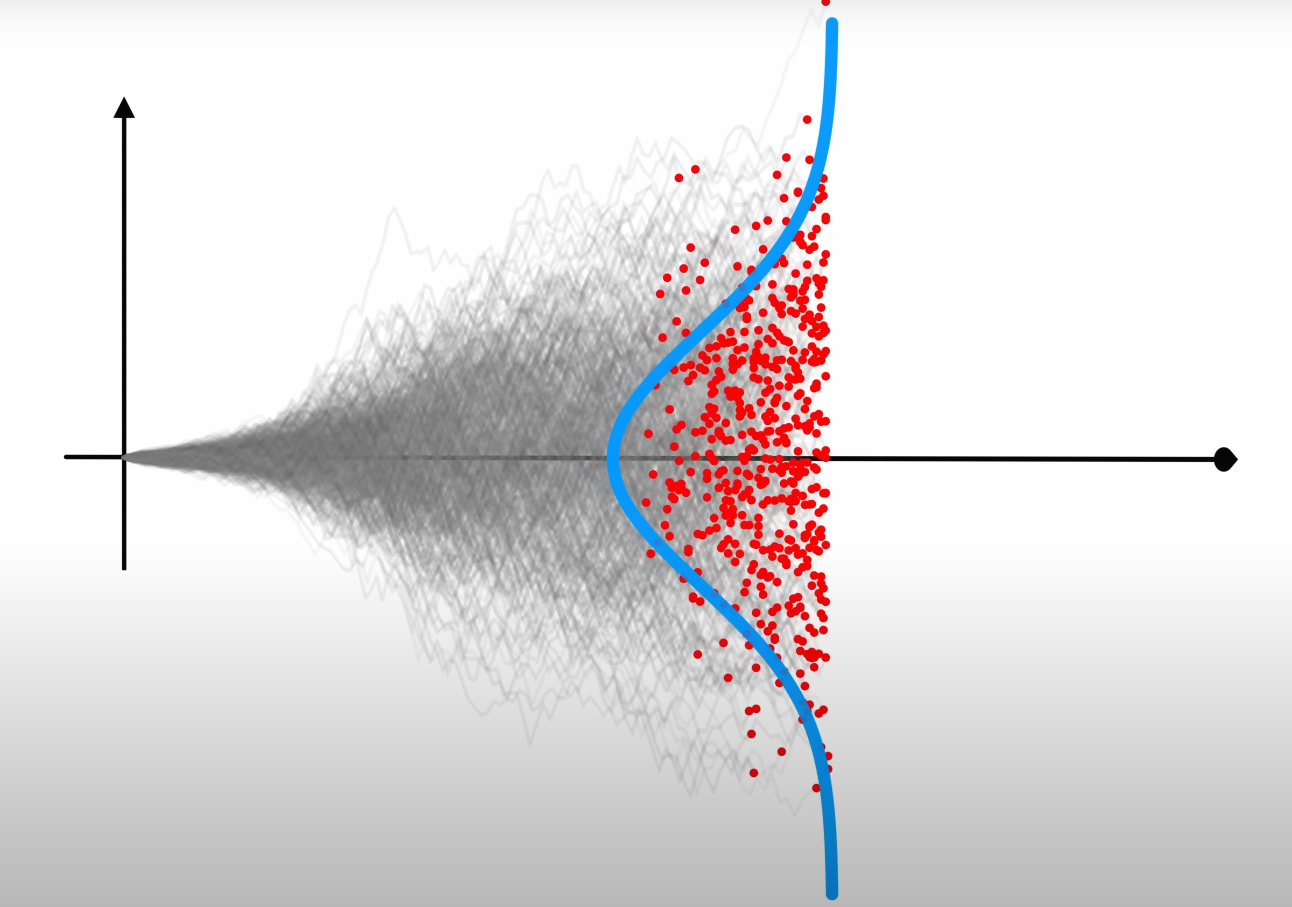
\includegraphics[width=0.5\linewidth]{img/Bachelier.png}
\caption{The stock price follows a normal distribution moving with time to the right.}
\end{figure}

An intuitive way to understand how a sequence of random walks produces a normal distribution is through the \textbf{Galton board}. In this device, balls randomly move left or right at each intersection, and the resulting pattern at the bottom naturally forms a bell-shaped curve as more balls are added.
\begin{figure} [H]
\centering
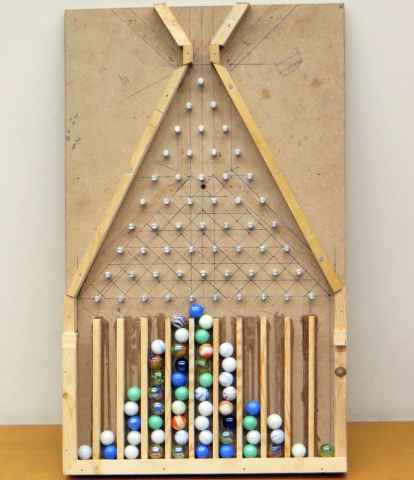
\includegraphics[width=0.5\linewidth]{img/Galton_Board_5.jpeg}
\caption{An example of Galton board.}
\end{figure}

Five years later, \textbf{Einstein} demonstrated that the same Gaussian law describes the probability distribution of particle displacements in \textbf{Brownian motion}, which is a particular solution of the \textbf{heat equation} first formulated by \textbf{Fourier} in 1822. In essence, Bachelier had anticipated that stock prices obey the same mathematical law governing the diffusion of heat from regions of high to low temperature:
\begin{equation}\label{eq:heat}
    \pdv{u}{t} = \alpha \pdv[2]{u}{x}
\end{equation} 

What we've learned to far:

\begin{table}[H]
\centering
\rowcolors{2}{gray!5}{white}
\begin{tabular}{@{}p{4cm}p{8.5cm}@{}}
\toprule
\rowcolor{gray!15}
\textbf{Model} & \textbf{Description} \\ \midrule
\textbf{Bachelier (1900)} &
Prices follow an \emph{arithmetic Brownian motion} and satisfy Fourier's heat equation. \\
\bottomrule
\end{tabular}
\caption{The Bachelier model (1900): the first stochastic model for asset prices.}
\end{table}


\subsection{The efficient Market Hypothesis (EMH)}
The \textbf{efficient-market-hypothesis} states that "\textit{asset prices reflect all available information}", basicaly you can't buy an asset and sell it immediately for profit.\\
This means that it is impossible for investors to consistently outperform the market through expert stock selection as any new information is quickly incorporated into stock prices (the more people try to predict and trade, the less predictable prices become).\\

 One can demonstrate that the EMH implies that the logarithm of stock prices follows a driven (with drift) random walk (omitted for brevity).

What we've learned so far:

\begin{table}[H]
\centering
\rowcolors{2}{gray!5}{white}
\begin{tabular}{@{}p{4cm}p{8.5cm}@{}}
\toprule
\rowcolor{gray!15}
\textbf{Model} & \textbf{Description} \\ \midrule
\textbf{Bachelier (1900)} &
Prices follow an \emph{arithmetic Brownian motion} and satisfy Fourier's heat equation. \\[3pt]
\textbf{Efficient Market Hypothesis (1960s)} &
Log-prices follow a driven random walk. \\ 
\bottomrule
\end{tabular}
\caption{From the Bachelier model to the Efficient Market Hypothesis.}
\end{table}

\subsection{Geometric Brownian Motion}

%\textbf{\large{Geometric Brownian Motion}}
\textbf{A geometric Brownian motion (GBM)} is a continuos-time stochastic process in which the logarithm of the random variable follows a Brownian motion with a drift (i.e. with a change of the average value of the random variable). \\
Using stochastic processes we can define stochastic differential equations (SDE), in which some terms and the solution are stochastic processes.
For example the SDE for the geometric brownian motion ($S_{t}$) is the following:
\begin{equation*}
    \dd S_{t} = \mu S_{t} \dd t + \sigma S_{t} \dd W_{t}
\end{equation*}
where $W_{t}$ is a Brownian motion, $\mu$ is the percentage drift and $\sigma$ is the percentage volatility.

\begin{figure} [H]
    \centering
    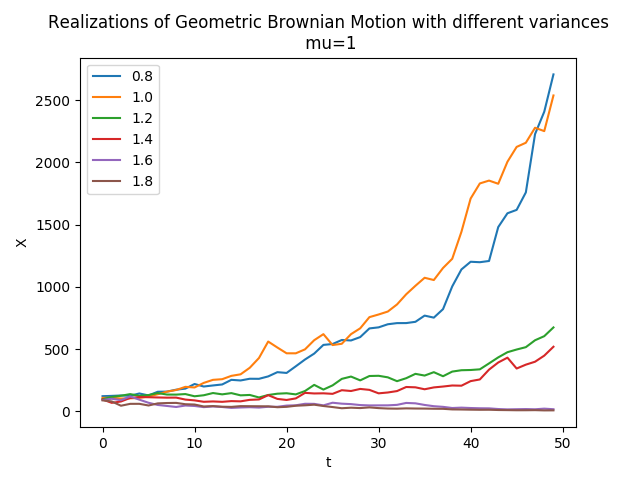
\includegraphics[width=0.75\linewidth]{img/GBM.png}
\end{figure}

\subsection{Black--Scholes--Merton Model (BSM)} 
If we take these assumptions on the market:
\begin{itemize}
    \item Ability to buy and sell any amount of the stock (without fees or costs);
    \item Ability to borrow and lend any amount at the riskless rate (without fees or costs);
    \end{itemize}
    and if it follows the efficient market hypothesis:
    \begin{itemize}
    \item There is a \textbf{risk-free interest rate} and it is \textbf{constant}. There is \textbf{no arbitrage} opportunity (there is no way to make a riskless profit exceeding the risk-free rate);
    \item The stock does not pay a dividend.
    \end{itemize}
Then not only the log return of the stock price follows a driven random walk (EMH), but the stock price follows a Geometric brownian motion:
\begin{equation*}
    \dd S = S \dd t + \sigma S \dd z
\end{equation*}
where $\dd S$ is the infinitesimal change in stock price, $S \dd t$ is the drift, and $\sigma S \dd z$ is randomness term, basically a brownian motion with drift.\\

After some number of steps, one should get the Black--Scholes/Merton equation:
\begin{equation} \label{eq:Black–Scholes}
    \pdv{V}{t} + rS \pdv{V}{S} + \frac{1}{2} \sigma^2 S^2 \pdv[2]{V}{S} - rV = 0
\end{equation}
Where $V$ is the price of the option, $S$ the price of the asset, $t$ the time, $\sigma$ is the volatility of the asset and $r$ is the risk-free interest rate. \\

In this case, since the log of the price follows an arithmetic brownian motion, it also solves the Fourier's heat equation.
We refer to Appendix~\ref{app:B} for the derivation transforming the Black--Scholes equation into the heat equation, and to Appendix~\ref{app:B_solution_Black-Scholes} for the detailed calculations leading to its solution.

What we've learned so far:

\begin{table}[H]
\centering
\rowcolors{2}{gray!5}{white}
\begin{tabular}{@{}p{3.8cm}p{8.2cm}@{}}
\toprule
\rowcolor{gray!15}
\textbf{Model} & \textbf{Description} \\ \midrule
\textbf{Bachelier (1900)} &
Prices follow an \emph{arithmetic Brownian motion} and satisfy Fourier's heat equation. \\[2pt]
\textbf{Efficient Market Hypothesis (1960s)} &
Log-prices follow a driven random walk. \\[2pt]
\textbf{Black–Scholes / Merton (1970s)} &
Prices follow a \emph{geometric Brownian motion}, hence log-prices satisfy Fourier's heat equation. \\ 
\bottomrule
\end{tabular}
\caption{From Bachelier to Black–Scholes: evolution of price modeling.}
\end{table}

